 The primary target of uncertainty quantification (UQ) is the characterization of the output of systems that exhibit non-deterministic behavior due to the presence of uncertainties of some kind \cite{xiu2010, eldred2009}.
 A multiprocessor platform is a prominent example of such a system, wherein the variability originates from, \eg, the semiconductor manufacturing process and operating environment.
 In particular, the uncertainty impacts power and, consequently, temperature, which are among the main concerns of multiprocessor system designs.
 As an example, consider a quad-core architecture subjected to uncertainty of the parameters that affect the leakage current.\footnote{The experimental setup is explained in \sref{experimental-results}.}
 Assume first that these parameters have nominal values. We can then simulate the system under a certain workload in order to observe the corresponding temperature.
 The result, labeled as ``Nominal'', is depicted in \fref{motivation-curve} where, for clarity, only two curves, corresponding to two processors, are presented (the two bottom blue lines). It can be seen that the temperature is always below $70^{\circ}$C. Now, let us assume a mild deviation of the parameters from the nominal values and run the simulation once again.
 The result is the ``Mild'' curves in \fref{motivation-curve} (the two middle orange lines); the maximal temperature is already above $80^{\circ}$C.
 Finally, we repeat the experiment considering a severe deviation of the parameters and observe the curves labeled as ``Severe'' in \fref{motivation-curve} (the two top green lines); the maximal temperature is almost $110^{\circ}$C.
 Imagine that the designer, when tuning the solution constrained by a maximal temperature of $80^\circ$C, was guided exclusively by the nominal parameters. In this case, even with mild deviations, the circuits might be burnt.
 The amount of burnt circuits depends on the statistical distribution of deviations.
 Such an uncertainty has to be addressed in order to pursue efficiency and robustness.
 Nevertheless, the majority of the literature regarding power-temperature analysis (PTA) ignores this important aspect, \eg, \cite{rao2009, rai2011, thiele2011, ukhov2012}.

\begin{figure}[bl]
  \vspace{-1.0em}
  \centering
  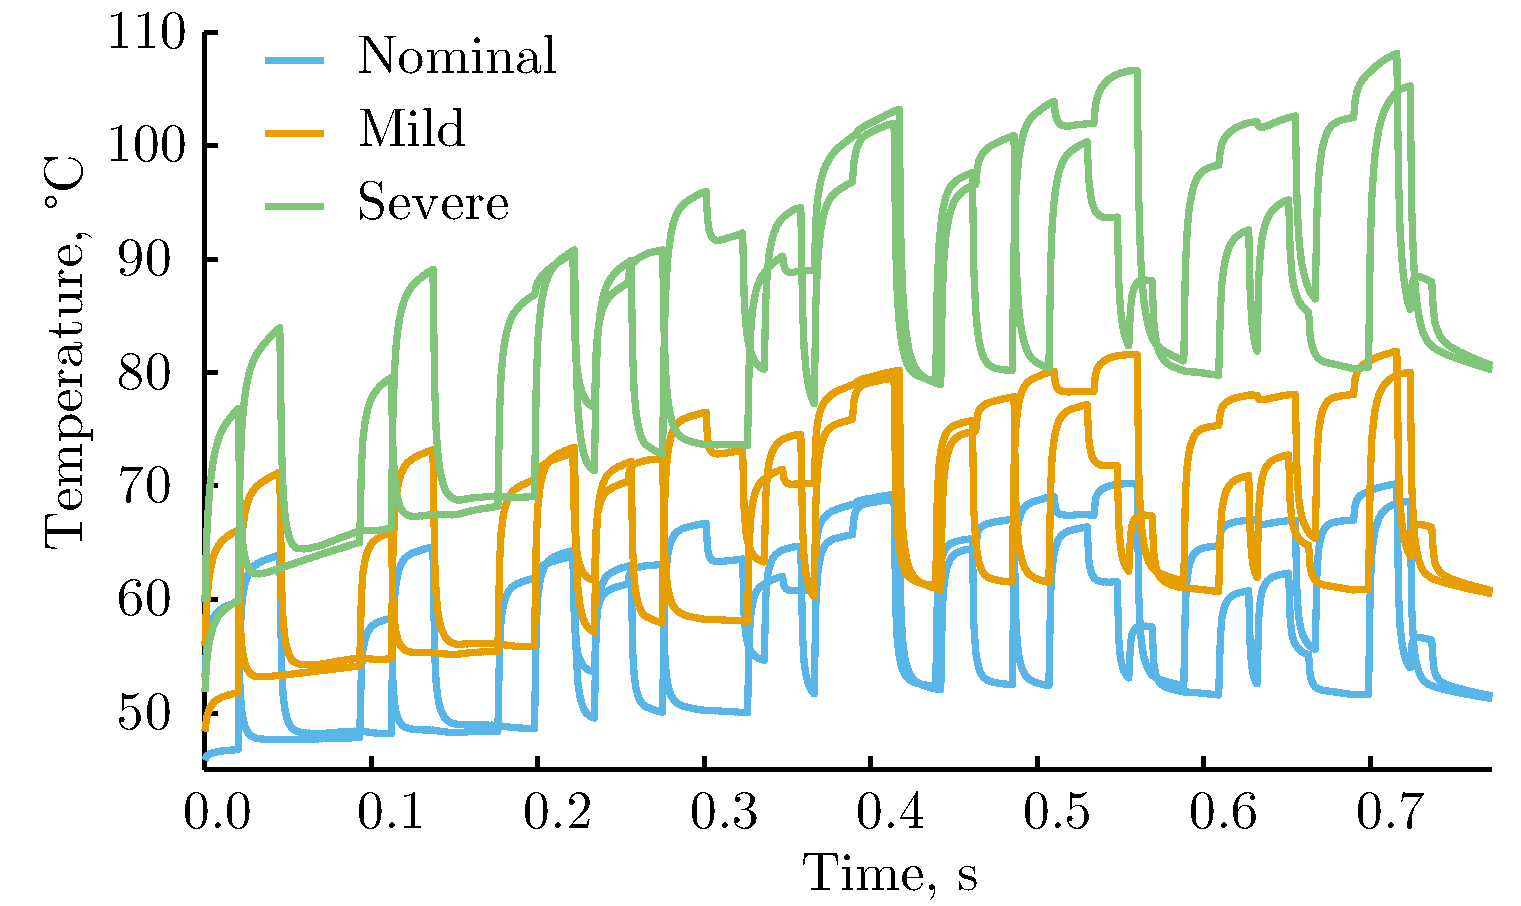
\includegraphics[width=1.0\linewidth]{include/assets/motivation-curve.pdf}
  \caption{Temperature fluctuation due to process variation.}
  \flabel{motivation-curve}
\end{figure}

